%% ****** Start of file apstemplate.tex ****** %
%%
%%
%%   This file is part of the APS files in the REVTeX 4.2 distribution.
%%   Version 4.2a of REVTeX, January, 2015
%%
%%
%%   Copyright (c) 2015 The American Physical Society.
%%
%%   See the REVTeX 4 README file for restrictions and more information.
%%
%
% This is a template for producing manuscripts for use with REVTEX 4.2
% Copy this file to another name and then work on that file.
% That way, you always have this original template file to use.
%
% Group addresses by affiliation; use superscriptaddress for long
% author lists, or if there are many overlapping affiliations.
% For Phys. Rev. appearance, change preprint to twocolumn.
% Choose pra, prb, prc, prd, pre, prl, prstab, prstper, or rmp for journal
%  Add 'draft' option to mark overfull boxes with black boxes
%  Add 'showkeys' option to make keywords appear
\documentclass[aps,prf,twocolumn,groupedaddress,showkeys]{revtex4-2}
%\documentclass[aps,prl,preprint,superscriptaddress]{revtex4-2}
%\documentclass[aps,prl,reprint,groupedaddress]{revtex4-2}

% You should use BibTeX and apsrev.bst for references
% Choosing a journal automatically selects the correct APS
% BibTeX style file (bst file), so only uncomment the line
% below if necessary.
%\bibliographystyle{apsrev4-2}

\usepackage{graphicx}
\usepackage{bm}
\usepackage{xcolor}

\begin{document}

% Use the \preprint command to place your local institutional report
% number in the upper righthand corner of the title page in preprint mode.
% Multiple \preprint commands are allowed.
% Use the 'preprintnumbers' class option to override journal defaults
% to display numbers if necessary
%\preprint{}

%Title of paper
\title{Turbulence modulation via dilute surfactant additives in experimental Taylor--Green flow}

% repeat the \author .. \affiliation  etc. as needed
% \email, \thanks, \homepage, \altaffiliation all apply to the current
% author. Explanatory text should go in the []'s, actual e-mail
% address or url should go in the {}'s for \email and \homepage.
% Please use the appropriate macro foreach each type of information

% \affiliation command applies to all authors since the last
% \affiliation command. The \affiliation command should follow the
% other information
% \affiliation can be followed by \email, \homepage, \thanks as well.
\author{Augusto H. P. Zanca}
\author{Yutaro Motoori}
\author{Susumu Goto}
%\email[]{Your e-mail address}
%\homepage[]{Your web page}
%\thanks{}
%\altaffiliation{}
\affiliation{Graduate School of Engineering Science, Osaka University}

%Collaboration name if desired (requires use of superscriptaddress
%option in \documentclass). \noaffiliation is required (may also be
%used with the \author command).
%\collaboration can be followed by \email, \homepage, \thanks as well.
%\collaboration{}
%\noaffiliation

\date{\today}

\begin{abstract}
% insert abstract here
Abstract here.
\end{abstract}

% insert suggested keywords - APS authors don't need to do this
%\keywords{}

%\maketitle must follow title, authors, abstract, and keywords
\maketitle

% body of paper here - Use proper section commands
% References should be done using the \cite, \ref, and \label commands
\section{Introduction\label{sec:Intro}}
% Put \label in argument of \section for cross-referencing
%\section{\label{}}
%\subsection{}
%\subsubsection{}

Since the discovery that trace amounts of dissolved polymer could lead to drag reduction in pipe flows~\cite{toms1948}, the use of additives for drag reduction in wall bounded flows has become established. Besides polymer solutions, it has since been discovered that self-assembling surfactant solutions share similar effects~\cite{lumley1969}, owing to the fact that dilute surfactant solutions can form wormlike micelles whole relaxation dynamics mimic that of polymer chains while resisting mechanical degradation. Beyond the applications of drag reduction, it has shown that viscoelastic additives are known to modulate turbulence more broadly, reshaping the energy spectrum and producing an elastic range governed by additive elasticity rather than inertial at the small scales~\cite{groisman2000,zhang2021sciadv}, with surfactant-specific micellar structures shown to alter vortex shedding and turbulence statistics directly~\cite{fukushima2022jfm}.

In spite of academic and commercial interest, comparatively few studies address the behavior of dilute surfactant solutions in the context of three-dimensional bulk turbulence, with most of the literature focused on wall-bounded or quasi-two-dimensional flows. This is in part related to the fact that the rheology of very dilute surfactant solutions remains difficult to pin down, with reported values of viscosity and relaxation time of CTAC/NaSal solutions (such as the considered in the present experiment) varying considerably between studies~\cite{kawaguchi2003rheological,zhang_effects_2008}. In spite of the diverging measurements and reports that some of the dilute solutions behave as a Newtonian fluid under rheological measuremen~\cite{kawaguchi2003rheological}, such solutions are known to produce measurable drag reduction~\cite{li_experimental_2008}, which further reinforces the need to analyze such solutions more in depth.

Motivated by this gap, here we present an experimental analysis of the turbulence generated by a four-rotor, Taylor—Green-like experiment using dilute CTAC solutions, in an attempt to characterize the modulation of turbulence caused by the addition of the surfactant across a wide range of Reynolds numbers for flows driven by inertial forcing.

\section{Experimental Device\label{sec:Exp}}

In the present study, we employ an experimental device designed to produce Taylor—Green-like forced turbulence on a laboratory setting. The apparatus, with schematic shown on figure~\ref{fig:schematic_1}, consists of a water tank with four rotors which are driven by a gear system and rotate in opposing directions in order to produce turbulence in the region between them (hereinafter simply denominated bulk), which is the target of our studies. Spatially-resolved measurements are obtained via 2D particle tracking (briefly described in section~\ref{sec:ptv}) via a traditional laser-sheet and high-speed camera combination, which are positioned as also shown in figure~\ref{fig:schematic_1} for the case of bulk imaging.

\begin{figure}
    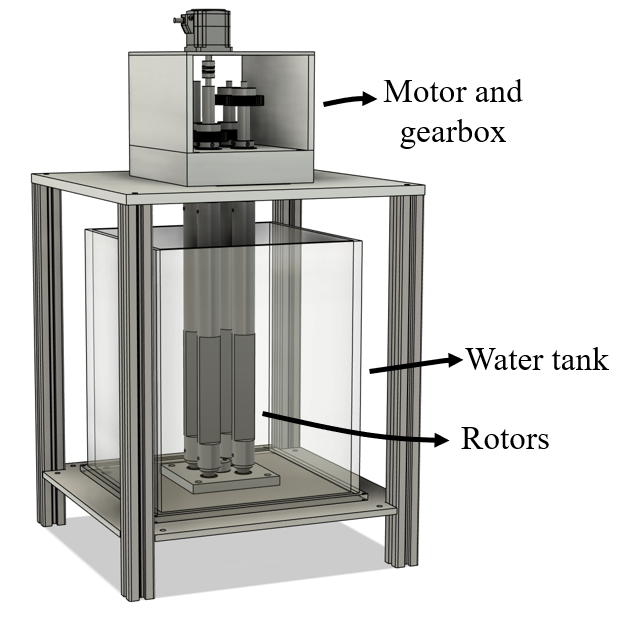
\includegraphics[width=0.45\columnwidth]{Images/cad_1.png}
    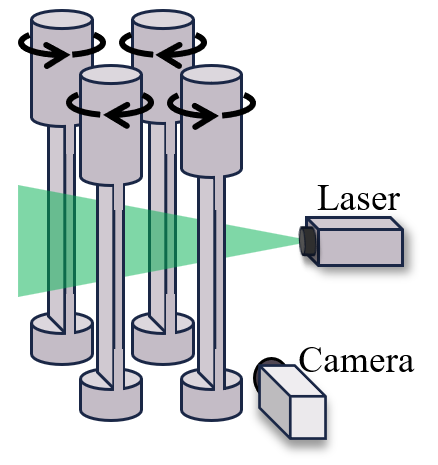
\includegraphics[width=0.4\columnwidth]{Images/schematic_1.png}
    \caption{CAD of the experimental device (left) and schematic showing normal orientation of camera and laser sheet, as well as direction of rotation of the rotors.}
    \label{fig:schematic_1}
\end{figure}

Aside from the imaging of the bulk region, it is also possible to change the relative orientations of the laser sheet and camera, and use a mirror to allow for top-down imaging of the region in the vicinity of the blades, as shown in the schematic of figure~\ref{fig:schematic_2}.

\begin{figure}
    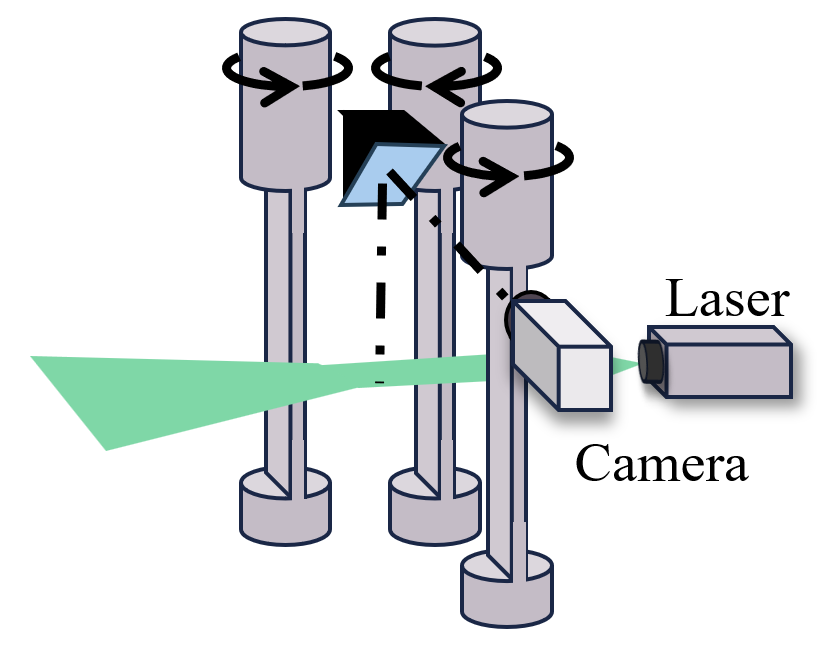
\includegraphics[width=0.4\columnwidth]{Images/schematic_2.png}
    \caption{Schematic of the altered orientation of camera and laser using mirror for imaging of the space between rotors. One of the rotors is omitted for clarity.}
    \label{fig:schematic_2}
\end{figure}

As shown in the schematics of figures~\ref{fig:schematic_1} and~\ref{fig:schematic_2}, the rotors themselves are shaped as blades with rectangular cross-section. While the design of the experimental device allows for the geometry of the rotors to be changed between cylinders and the carved blades, the use of the latter allows us to isolate inertial forcing in the driving of the flow, and therefore ignore boundary-layer effects which would be present in the case of viscous driving which happens when cylindrical rotors are used. Additionally, the rotation direction is such that mean stretching of the flow happens in the out-of-plane component of the camera image (when imaging the bulk region in the vertical plane), and is accompanied by the formation of secondary vortices as shown in previous numerical studies~\cite{goto2017hierarchy}. For simplicity, the carved rotors will hereinafter simply be denominated blades. 

While not shown in the schematics, the experimental device is also encased in thermal insulation and connected to an air-processor system. By controlling the temperature of the surrounding air, the water temperature was maintained at approximately 26 $^\circ$C over the course of the experiments.

\subsection{Data measurement and reduction\label{sec:ptv}}

As previously mentioned, processing of the obtained images to calculate the velocity fields is conduced via a particle tracking velocimetry (PTV) code developed in-house. Although the details of the algorithm are out of the scope of the current document, the code is built as a collection of previously established methods. For the detection of tracer particles from the images, we employ a variation of the Iterative Particle Reconstruction (IPR) method, which is commonly employed for  volumetric particle tracking as part of the Shake-the-Box method~\cite{ipr_jahn2021}. The tracking of detected particle positions between the video frames is carried out by a variation of the Polar Coordinate-System Similarity (PCSS) method~\cite{PCSSimproved}.

Before the calculation of the final velocity vectors through finite differencing, the trajectories are filtered according to a Wiener Filter~\cite{wiener1949extrapolation} which is calculated from the spectra of position of the obtained trajectories. The filtering is done in order to avoid the effect of the noise floor in the calculation of the velocities. (need to revisit this) (also need to mention the interpolation that is done before the spatial average) \textcolor{red}{also supplement this with the explanation of the uncertainty calculation and all}.

\subsection{Surfactant solutions}


The surfactant used in the current study was the cationic surfactant cetrimonium chloride (CTAC), with the addition of sodium salicylate on a molar ratio of approximately 4:1 to provide counterions. The solution is prepared by mixing the adequate amounts of surfactant and salt with tap water and then agitating in a magnetic stirrer over a period of at least 12 hours, after which the resulting solution is added to the experimental device.  For simplicity, the surfactant and salt solution are hereinafter denominated simply as the CTAC solution, with the solution concentration corresponding exclusively to the concentration of the surfactant counterpart.

For the analysis of the effect of solution concentration on the results, three CTAC solutions of concentrations of 33 ppm, 50 ppm, and 100 ppm were  prepared. As previously mentioned, rheological measurements of such dilute solutions have historically yielded diverging results~\cite{kawaguchi2003rheological,zhang_effects_2008}, meaning that to the best of the author's knowledge, there is no precise measurement of the properties such as the relaxation time of micellar structures under these conditions. 

Moreover, the molar ratio of 4:1 chosen for the current study differs from that of the aforementioned measurements, as well as that of drag reduction studies~\cite{li_experimental_2008}. Although numerical studies have reported that such high molar ratios can lead to the formation of branched structures and loss of viscoelasticity~\cite{wang_study_2017}, such claims have been made for solutions of much higher concentrations. In the experience of the authors, this effect is not as pronounced in the case of dilute solutions, and the use of a high molar ratio has been chosen to favor the formation of longer micellar structures.

In spite of these divergences, it can be expected from the aforementioned studies that this relaxation time should be in the order of $10^{-1}$ seconds. Since the relaxation time cannot be precisely known beforehand or independently controlled over a wide range, a sweep over the Weissenberg \textcolor{red}{you need to define what is the weissenberg number bro} number is instead achieved by changing the Reynolds number of the generated turbulence. For each of the prepared solutions, the rotation rate of the blades is changed $2^{-3}$ to $2^4$ Hz in powers of two. Exclusively for the 100 ppm solution \textcolor{red}{say how the rotation rate was reduced further}. Although it is debatable whether the flow generated in the case of the lower rotation rates can be denominated turbulent, it remains chaotic and unsteady, so such cases are still useful in the determination of the effect of surfactant addition on such unsteady but low Reynolds number types of flows. 

The next section describes briefly the characterization of the turbulence generated in the current experimental device for the case of Newtonian fluid.

\section{Turbulence Characterization\label{sec:Turbchar}}

Considering the unique nature of the current experimental apparatus, we conduct a characterization of the turbulence generated in the case of Newtonian flow as a function of the rotation rate of the blades. Although the generated turbulence is anisotropic, turbulent statistics become approximately homogeneous in the vicinity of the stagnation point of the mean flow in the center of the experiment. Owing to this, the statistics are computed as spatiotemporal averages over the duration of the experiments. Figure~\ref{fig:turbchar_uvprime} displays the velocity fluctuation RMS as a function of the blade rotation speed, demonstrating that there ins an approximately linear trend, with the ratio between the two components remaining somewhat constant as well. Note that the turbulent intensity is more pronounced in the horizontal direction, consistent with the primary forcing direction of the blades.

\begin{figure}
    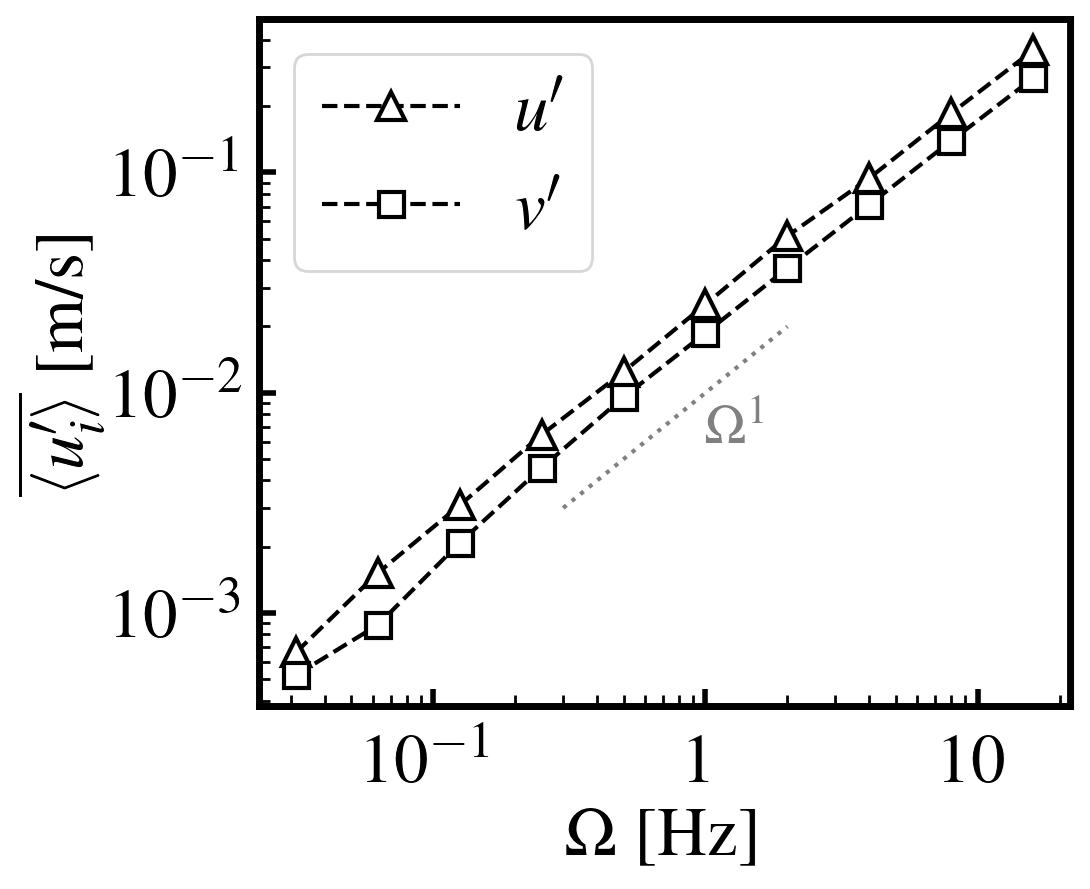
\includegraphics[width=0.6\columnwidth]{Images/uvprime_plot.png}
    \caption{Spatially averaged velocity fluctuation RMS in the bulk as a function of rotation rate of the agitator blades..}
    \label{fig:turbchar_uvprime}
\end{figure}

Although direct measurement of the dissipation range is not feasible under current experimental conditions, the turbulent dissipation can be estimated through the third-order structure function, as shown in figure~\ref{fig:turbchar_thirdordervsf}. Note that although the generated turbulence is anisotropic, the results of figure~\ref{fig:turbchar_thirdordervsf} indicate that the dissipation rate is approximately independent of the measurement direction, which helps to validate the obtained results \textcolor{red}{is this correct?}. In all the plots, the increase in the value of the structure function as the separation distance reaches the smallest values is caused by the finite depth-of-correlation and the nature of planar imaging, as well as the fact that no interpolation of the instantaneous velocity fields is used for the calculation of these statistics.

For the cases of high rotation rate, the appearance of a horizontal region indicates that an inertial range is well-defined, and the dissipation rate can be taken as the average across this region. For the lower rotation rates, the Reynolds number is too low for the appearance of a defined inertial range, and the extraction of a representative value of dissipation is more difficult. For consistency between the cases, we consider the average value of the normalized third-order structure function between the separations of $r=3$ mm and $r=20$ mm as the dissipation value. These representative values are represented as the dotted lines of figure~\ref{fig:turbchar_thirdordervsf}.

\begin{figure}
    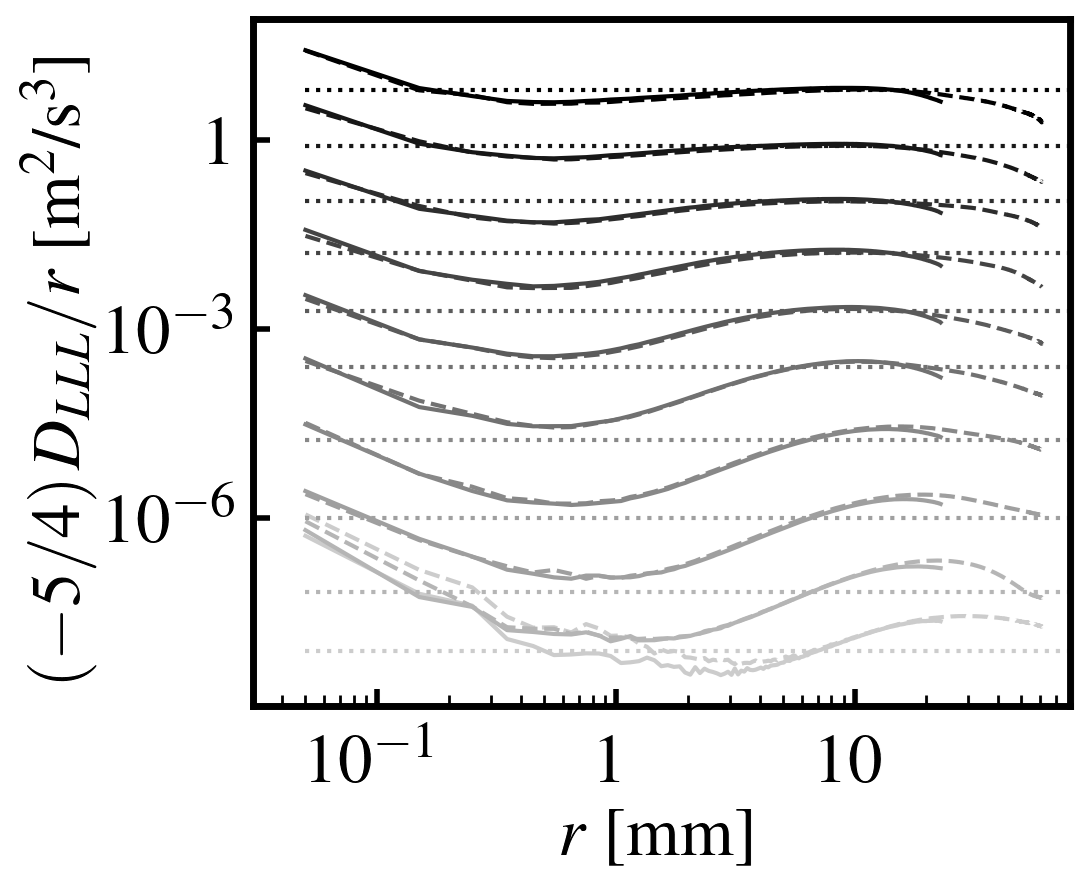
\includegraphics[width=0.6\columnwidth]{Images/thirdordervsf.png}
    \caption{Normalized third-order structure function for different rotation rates. Darker lines represent a higher rotation rate.}
    \label{fig:turbchar_thirdordervsf}
\end{figure}

From these results, we can then obtain the approximate Kolmogorov lenghtscale and timescale for each of the cases, as shown in figure~\ref{fig:turbchar_etatau}. From these results, the estimated Kolmogorov lenghtscale provides us with an additional clue as to why it is not possible to directly measure the dissipation range, considering that these scales become smaller than the depth-of-correlation of the current imaging system for most rotation rates. Additionally, wide range of the estimated timescales indicate that a wide range of Weissemberg numbers should be obtained regardless of the fact that the relaxation time of the surfactant solutions is not precisely known.

\begin{figure}
    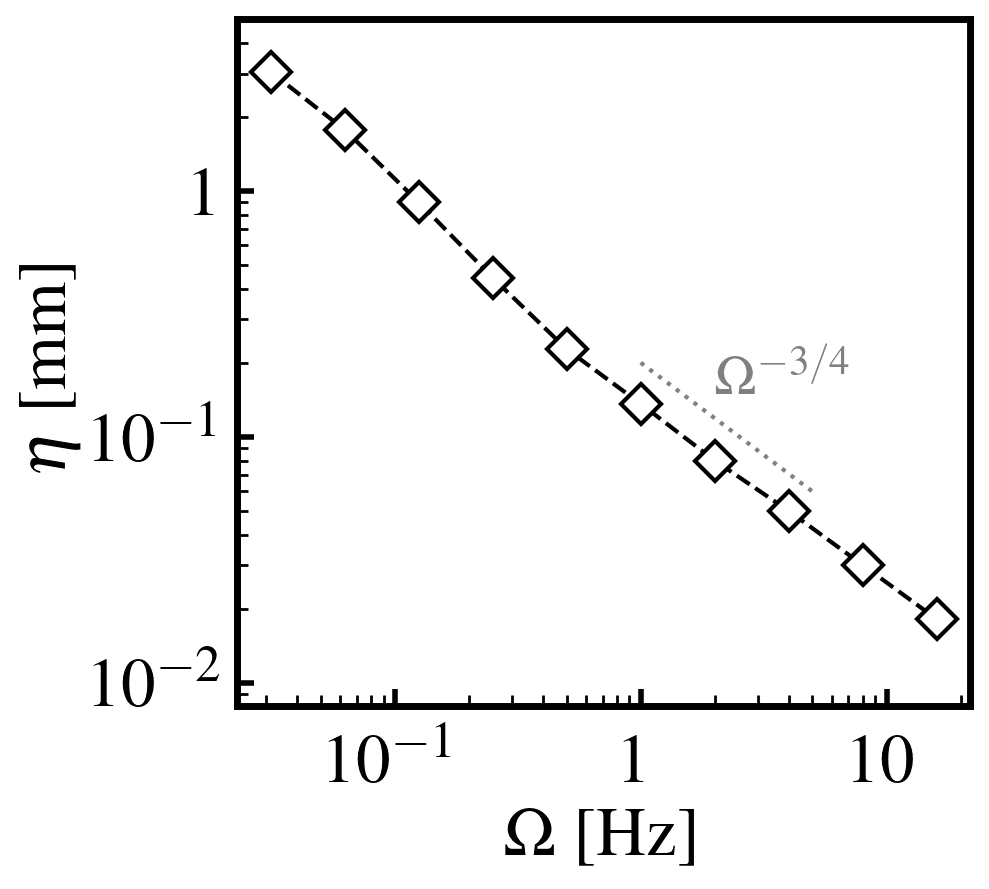
\includegraphics[width=0.45\columnwidth]{Images/eta_plot.png}
    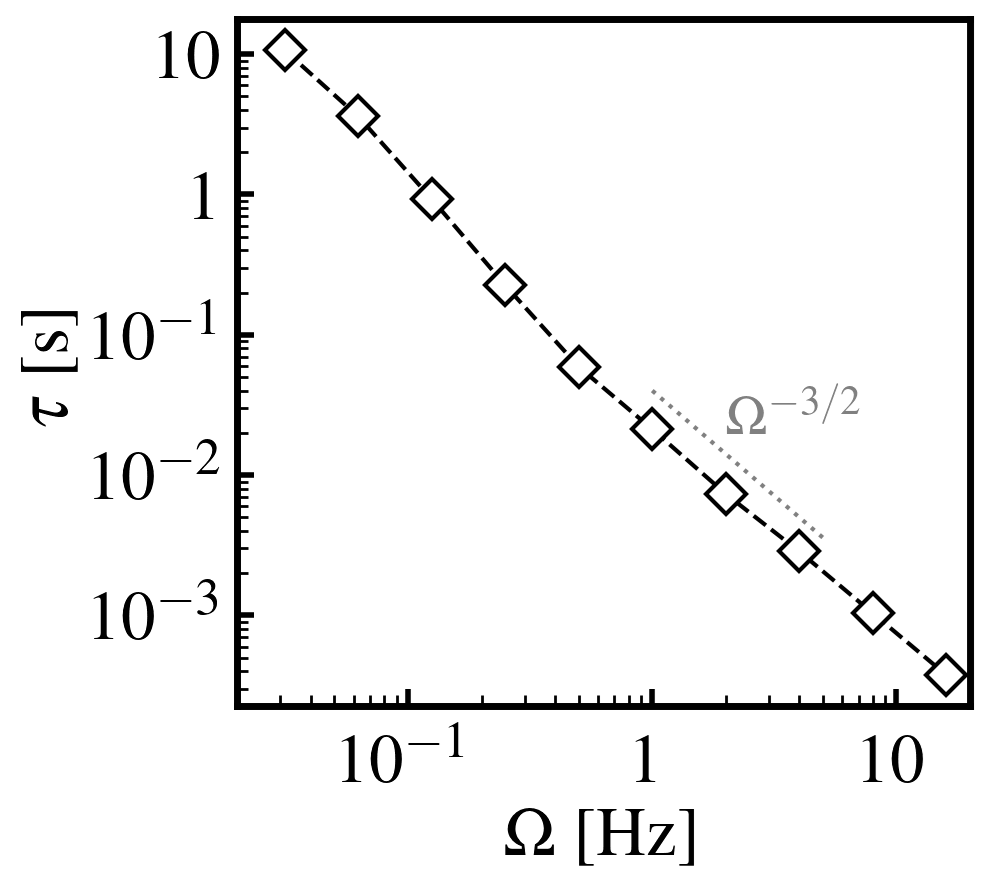
\includegraphics[width=0.45\columnwidth]{Images/tau_plot.png}
    \caption{Kolmogorov lenghtscale and timescale as a function of rotation rate of the agitator blades.}
    \label{fig:turbchar_etatau}
\end{figure}

\section{Results\label{sec:Res}}

\section{Conclusions\label{sec:Conclus}}

% If in two-column mode, this environment will change to single-column
% format so that long equations can be displayed. Use
% sparingly.
%\begin{widetext}
% put long equation here
%\end{widetext}

% figures should be put into the text as floats.
% Use the graphics or graphicx packages (distributed with LaTeX2e)
% and the \includegraphics macro defined in those packages.
% See the LaTeX Graphics Companion by Michel Goosens, Sebastian Rahtz,
% and Frank Mittelbach for instance.
%
% Here is an example of the general form of a figure:
% Fill in the caption in the braces of the \caption{} command. Put the label
% that you will use with \ref{} command in the braces of the \label{} command.
% Use the figure* environment if the figure should span across the
% entire page. There is no need to do explicit centering.

% \begin{figure}
% \includegraphics{}%
% \caption{\label{}}
% \end{figure}

% Surround figure environment with turnpage environment for landscape
% figure
% \begin{turnpage}
% \begin{figure}
% \includegraphics{}%
% \caption{\label{}}
% \end{figure}
% \end{turnpage}

% tables should appear as floats within the text
%
% Here is an example of the general form of a table:
% Fill in the caption in the braces of the \caption{} command. Put the label
% that you will use with \ref{} command in the braces of the \label{} command.
% Insert the column specifiers (l, r, c, d, etc.) in the empty braces of the
% \begin{tabular}{} command.
% The ruledtabular enviroment adds doubled rules to table and sets a
% reasonable default table settings.
% Use the table* environment to get a full-width table in two-column
% Add \usepackage{longtable} and the longtable (or longtable*}
% environment for nicely formatted long tables. Or use the the [H]
% placement option to break a long table (with less control than 
% in longtable).
% \begin{table}%[H] add [H] placement to break table across pages
% \caption{\label{}}
% \begin{ruledtabular}
% \begin{tabular}{}
% Lines of table here ending with \\
% \end{tabular}
% \end{ruledtabular}
% \end{table}

% Surround table environment with turnpage environment for landscape
% table
% \begin{turnpage}
% \begin{table}
% \caption{\label{}}
% \begin{ruledtabular}
% \begin{tabular}{}
% \end{tabular}
% \end{ruledtabular}
% \end{table}
% \end{turnpage}

% Specify following sections are appendices. Use \appendix* if there
% only one appendix.
%\appendix
%\section{}

% If you have acknowledgments, this puts in the proper section head.
%\begin{acknowledgments}
% put your acknowledgments here.
%\end{acknowledgments}

% Create the reference section using BibTeX:
\bibliography{main}

\end{document}
%
% ****** End of file apstemplate.tex ******

